\section{The competition}
\label{competition}
\noindent
The initial goal for Naiad, after its completion, is to compete in RoboSub 2015. Since the missions are similar from one year to another the tactics and analysis is based on the rules from the rules and missions document of RoboSub 2014.\cite{robosubrules}
	\subsection{Overview}
\noindent 
On the competition website it is stated that the goals for the competition is to provide students with the opportunity to experience system engineering, accomplish realistic missions with AUVs and furthermore to build on the relationship between the young engineers and the developers and producers of different autonomous vehicle technologies.\cite{robosub}

There are two main parts to how the team and robot is judged. From their submitted journal paper, website and movie the team is scored with a subjective score from the judges. The team is scored with a performance measure from their execution of the missions. The sum of these scores result in the final score.
	\subsection{Subjective judging}
\noindent The rules state that each vehicle will be subject to a static judging during the competition. The judges evaluate the vehicle's technical merit, safety as well as its craftsmanship.  In the subjective and static judgings the following is measured.  

\begin{itemize}\itemsep1pt \parskip0pt \parsep0pt
\item Utility of website
\item Technical merit
\item Written style
\item Technical accomplishments
\item Craftsmanship
\item Team uniform
\item Team Video
\item Discretionary static points
\end{itemize}
All of these can give a total of 400 points. 

Weight, size of the AUV and size of the markers and torpedoes will also be measured in the static judging. 
	\subsection{Missions}
\noindent The following missions are described in the rules of RoboSub 2014 \cite{robosubrules}.

The team has 15 minutes to perform all missions, finishing before will give bonus points, T minutes left will give $T*100$ in bonus points. 

The first mission is always to pass through the validation gate, if this is done, the AUV is free to continue with the rest of the missions. 100 points is rewarded for passing through the gate, another 150 points is rewarded for maintaining a fixed heading through the validation gate. 
		\subsubsection{Path}
\noindent The path consists of segments leading the way to the different missions. The mission is to always follow the path to the next mission. The path segments are 0.15 m wide by 1.2 m long sections that are covered in orange duck tape. 100 points per followed segment will be awarded. 
		\subsubsection{Control Panel}
\noindent In this mission there are three buoys, two of which will be self-illuminated with high power RGB LEDs (RGB-buoy). These RGB-buoys will cycle through each of these three colours every 5 seconds. The aim is to bump these to get a desired colour. The desired colour will be presented at the start of the competition. The first bump at a buoy will stop it from toggling between the different colours, every subsequent bump after that will toggle the buoy through the colors. 
This mission will award a maximum of 1500 points. 400 points for bumping at least one of the buoys, either one of the RGB-buoys or the solid coloured bouy. For setting one of the RGB-buoys to the correct colour, 700 points will be rewarded. For setting both the RGB-buoys to the desired colour 1500 points will be rewarded. 
		\subsubsection{Maneuvering}
\noindent The maneuvering mission goal is to pass a PVC-construction. The AUV should either pass over it or around it. The construction for this mission can be found in figure \ref{maneuvering_mission}.
\begin{figure}[!ht]
	\begin{center}
		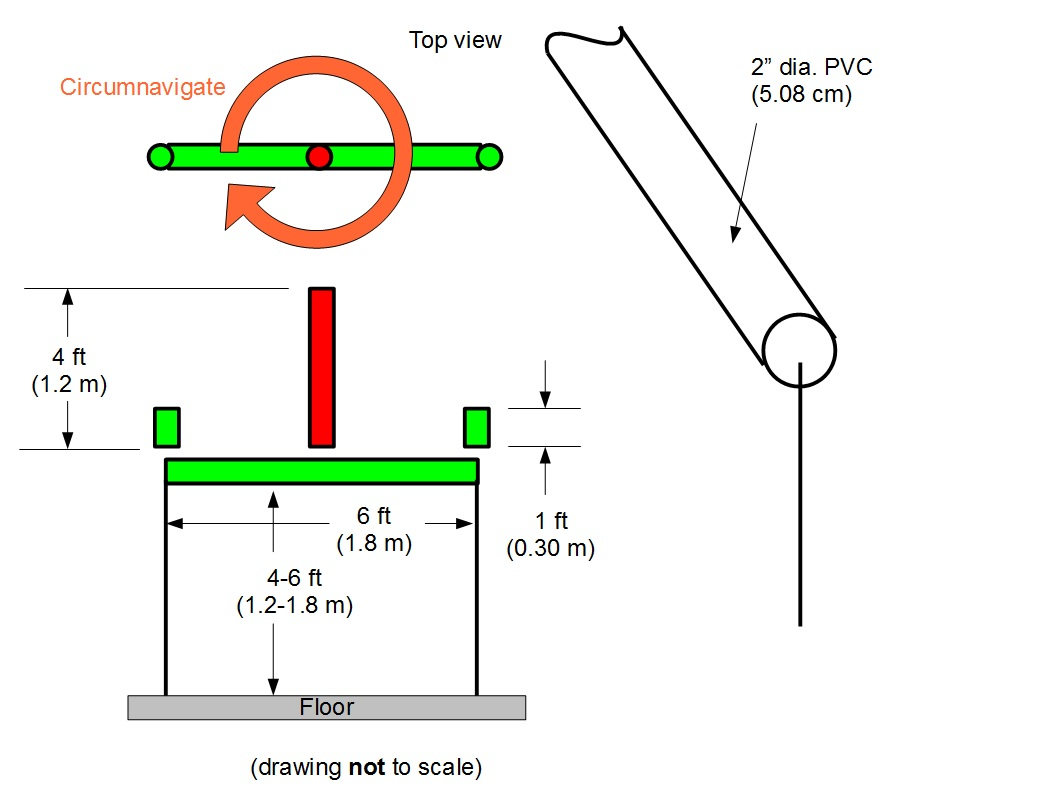
\includegraphics[width=80mm]{./Images/Competition/Maneuvering_mission.jpg}
		\caption{Design of the construction for the maneuvering mission}
		\label{maneuvering_mission}
	\end{center}
\end{figure}
There are two different ways to score in this mission. One where the AUV should pass over the horisontal section, between the red riser in the center and the green risers on the outer end of the horisontal section. This gives 600 points if more than half of the AUV is passing below the highest point of the center riser. If the AUV passes higher than that, it is awarded with 400 points. 
The other way is to circumnavigate the center riser. The method and orientation for the circumnavigation is optional for the teams. The AUV may also extend further out than the Green risers. To score using this method, the AUV should do a full 360\degree rotation around the center riser. If the AUV is able to do so with more than half the vehicle above the top end of the center riser, 1000 points are awarded. If it completes the circumnavigation with at least half the vehicle under the top of the center riser, 1400 points is awarded.
		\subsubsection{Landing Site}
\noindent The Landing Site consists of four black boxes placed in a square with white borders. The boxes are 30 cm wide and 60 cm long and each box has a 15 cm wide white border. The different bins will contain different silhouettes, as shown in fig. \ref{landingsite_silhouettes}.  
\begin{figure}[!ht]
	\begin{center}
		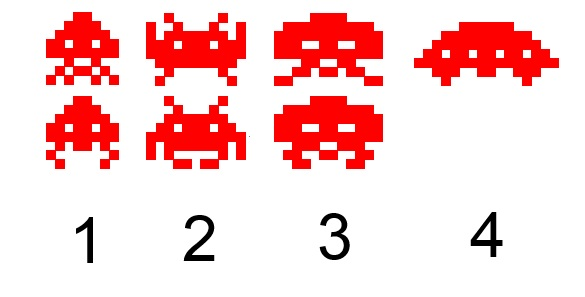
\includegraphics[width=80mm]{./Images/Competition/landingsite_silhouettes.jpg}
		\caption{The possible silhouettes for the Landing Site mission}
		\label{landingsite_silhouettes}
	\end{center}
\end{figure}
Only one silhouette from each column will be in the four bins. One of the silhouettes in the boxes will be designated as the primary target and another will be designated as the secondary target. Teams are awarded the most points for dropping one marker in the primary target and one in the secondary, 1400 points per marker. Half the points, 700 points per marker, is awarded for dropping markers in any bin. 
		\subsubsection{Brunch}
\noindent The Brunch mission is to fire the two torpedoes into the right holes of a green, square board. The board will have a picture of a spaceship. Above the spaceship there will be four 12.7 cm circular cutouts with 17.8 cm black borders. Below the spaceship two bigger holes can be found, 25.4 cm cutout circles with 30.5 cm black borders around them. During each run, two of the smaller circles and one of the larger will be covered, leaving 3 open holes. The goal is to fire the torpedoes through each of the smaller cutouts, however points will be rewarded for firing through any hole. Getting a torpedo through the big hole gives 700 points per torpedo, firing a torpedo through one of the smaller holes gives 1000 per torpedo. To receive full marks, both the smaller targets has to be hit individually, this award the team 2500 points. 
		\subsubsection{Reroute Power}
\noindent The Reroute Power mission consists of a 91 cm yellow square with eight blue circles distributed evenly in a square 15 cm in from the border of the square. Four red power pins will be arranged on the eight blue circles so that 4 circles has power pins and 4 are empty. The goal is to remove one pin and place it in an unoccupied blue circle. This will be rewarded with 1000 points per power pin. Just removing one power pin will result in 300 points per power pin. Placing the power pin back in it's previous position provides 700 points per power pin. Maximum score for this mission is 4000 points. 
		\subsubsection{Recovery Area}
\noindent There are two separate parts to this mission, where both needs to be done consecutively for the team to receive all points. 

The constructions for this task are two octagons constructed from PVC pipes, three moon rocks in the colour grey, three cheese structures in the colour green and a sample box. The octagon will be 2.7 m at its widest. The moon rock will be a 15.2 cm cube and the cheese will be a 10.4 cm high. The Collection Site is a 1.2 m square that is 7.6 cm high. There are also two pingers, located directly under the structure holding the Sample boxes, the octagons is floating on the surface directly above this structure. This is called the Recovery area, from which there is a path segment pointing directly at the Collection Site. At the start of each run one of the two pingers will be turned on and the moon rocks and cheeses will be positioned at the Collection Site. The team captain can choose to switch the active pinger, this should then be done when the object has been collected but before the AUV has surfaced. 

Points are distributed in three different categories for this mission. For surfacing, the AUV should surface with no portion of itself outside the octagon. Surfacing in the wrong octagon is rewarded 500 points whilst surfacing in the right octagon rewards the team with 2000 points. To receive full marks for recovery, the AUV has to capture the object so that it is constrained in at least three degrees of freedom when the AUV surfaces. The maximum reward for recovery is 1200 points. Dropping the object should be done from the surface, ability to do so is rewarded with 500 points. For hitting the Sample box with said object, teams are rewarded another 1000 points per object. Ability to put more than one similar object in the same sample box doubles the points, as well as the ability to put objects in both sample boxes. 

	\subsection{Tactics and analysis}
\noindent
The missions were categorised into three different categories; solved, potential and not possible. The idea is that the missions listed as solveable are the ones where only software development is needed at this stage, potential is the ones where we have all the hardware but it is not finalised. The missions listed as not possible are the ones where there is not even a clear solution for the hardware required for this mission. Since there is no design for the manipulator at this moment, the missions requiring this are listed as not possible. 
\subsubsection*{Solveable}
\begin{itemize}
\item Gate - the gate rewards points for passing through, and additional points for maintaining a fixed heading through it. To make sure to maintain a fixed heading the vision system should be used. 
\item Control Panel - the control panel can give the team a maximum of 1500 points. For this the requirement is the vision system. 
\item Maneuvering - The only requirement for this is the vision system. 
\item Path - The only requirement for the path is the vision system. 
\end{itemize}
\subsubsection*{Potential}
\begin{itemize}
\item Landing site - To succeed with this mission both vision system and a system for releasing the markers need to be working. 
\item Surface - To do this the AUV must be able to find the pinger using the hydrophones. 
\item Brunch - To do this the vision system and a system for firing torpedoes is needed. 
\end{itemize}
\subsubsection*{Not possible}
\begin{itemize}
\item Reroute power - Rerouting power requires both the vision system and the manipulator (gripper).  
\item Collecting objects - Collecting objects requires both the vision system, the manipulator and the hydrophones to be working. 
\end{itemize}

According to this a rough guesstimate would be that Naiad could receive 2250 points, doing the missions that are listed as solveable. If the missions listed as potential were to be solved before the competition, an additional 3400 points.